\documentclass[11pt, oneside,margin=1in]{article}   	% use "amsart" instead of "article" for AMSLaTeX format
\usepackage{geometry}                		% See geometry.pdf to learn the layout options. There are lots.
\geometry{letterpaper}                   		% ... or a4paper or a5paper or ... 
%\geometry{landscape}                		% Activate for rotated page geometry
%\usepackage[parfill]{parskip}    		% Activate to begin paragraphs with an empty line rather than an indent
\usepackage{graphicx}				% Use pdf, png, jpg, or eps§ with pdflatex; use eps in DVI mode
								% TeX will automatically convert eps --> pdf in pdflatex		
\usepackage{amssymb}

%SetFonts

%SetFonts
\usepackage{comment}
\usepackage{url}
\usepackage{amsmath,amsthm}
\newtheorem{remark}{Remark}
\newtheorem{lemma}{Lemma}
\newtheorem{theorem}{Theorem}
\newcommand{\E}{\mathbb{E}}

\title{\vspace{-.7 in} Rebates in Supply Chains}
\author{Nick Arnosti}
\date{April 13, 2018}							% Activate to display a given date or no date

\begin{document}
\maketitle

\begin{abstract}
Textbook publishers frequently agree to buy unsold textbooks back from campus bookstores, presumably in an effort to increase order quantities and sales. We consider a model in which publishers jointly set wholesale prices and rebate policies, and bookstores solve an associated Newsvendor problem. We solve for optimal wholesale prices, rebates, and order quantities, and identify two key insights. First, when the publisher is a monopolist, it is optimal to set wholesale prices such that bookstores make almost no profit from each sale, but to offer a full rebate. Second, increased competition causes the publisher to lower  wholesale prices and offer a less generous rebate policy -- in the extreme case of a perfectly competitive market, wholesale prices are equal to the marginal cost of provision and no rebate is offered. %Furthermore, in competitive markets, rebates are relatively more generous for high-margin products.
\end{abstract}
%\section{}
%\subsection{}



\section{Model}

To highlight the generality of the model, in what follows we refer to the publisher as a ``supplier", and the bookstore as a ``retailer."


A supplier can provide a retailer with items to sell. The retail price of the item is fixed to be $p$, and at that price, customer demand for the item (from the retailer) is distributed according to a known distribution with cdf $F$.\footnote{For simplicity of notation, in what follows we assume that $F$ is continuous and strictly increasing on some interval $[\underline{d},\overline{d}) \subseteq [0,\infty)$, with $F(\underline{d}) = 0$ and $F(\overline{d}) = 1$, so that $F^{-1}$ is well-defined.} The marginal cost to the supplier of providing an additional book is $c_m$ (this may account for manufacturing and/or shipping costs), and the retailer incurs a holding cost of $c_h$ for each item purchased. We assume that $p > c_m + c_h$ and define the {\em margin} of the product to be $M = (p - c_m-c_h)/p$ (this is the percentage of the sale price that serves as profit for either the supplier or the retailer). A reader looking for the ``simplest" version of this model can assume $p = 1$ and $c_h = 0$, as this is sufficient to reveal all major insights. The game is as follows:
\begin{enumerate}
\item The supplier chooses a wholesale price $w$, and a rebate $r$ that will be offered for each unsold item.
\item The retailer chooses an order quantity $q$.
\item Demand $d \sim F$ is realized, and any unsold books are returned to the supplier.
\end{enumerate}
The utilities of the supplier and retailer given wholesale price $w$, rebate $r$, order quantity $q$ and demand $d$ are respectively
\begin{align*}
U_S(w,r,q,d) & = (w - c_m) q - r \max(q-d,0)\\
U_R(w,r,q,d) & = p \min(q,d) + r \max(q-d,0) - q(w+c_h) \\
 & = q(p - w - c_h)  - (p-r) \max(q-d,0).
\end{align*}
Both the supplier and retailer are risk-neutral. In what follows, we make use of the following identity.
\begin{equation} \E_{d \sim F} [\max(q-d,0)] = \int_0^q F(x) dx \end{equation}

We assume that whenever the retailer is indifferent between different order quantities, the supplier chooses which of these quantities will be ordered by the retailer.\footnote{This is analogous to letting the mechanism designer select their preferred equilibrium in auction theory. It ensures that the supremum of the supplier's expected profit is attainable. If instead we assumed that the retailer chose among optimal order quantities antagonistically, then the supplier could get arbitrarily close to this supremum by using small deviations from the policies stated in this paper.}


\section{Monopolist Supplier}

As is typical with Stackelberg games, we solve by backwards induction. Given wholesale price $w$ and rebate $r \leq w + c_h$,\footnote{If $r > w + c_h$, then the retailer prefers to order as many items as possible, as unsold books are profitable.} a retailer that orders quantity $q$ earns expected reward of
\begin{equation} \E_{d \sim F} [U_R(w,r,q,d)] = q(p - w - c_h) - (p - r) \int_0^{q} F(x)dx \label{eq:ur} \end{equation}
If $p > r$, this has a unique local maximum, given by\footnote{In the language of the standard Newsvendor problem, the retailer faces overage cost $c_o = w + c_h - r$ and underage cost $c_u = p - w - c_h$, and chooses an order quantity $q$ such that $F(q) = \frac{c_u}{c_u+c_o}$. If $p = w + c_h = r$, then $c_u$ and $c_o$ are undefined, and the retailer is indifferent between all order quantities.}
\begin{equation} q(w,r) = F^{-1}\left( \frac{p - c_h - w}{p - r} \right). \label{eq:qwr} \end{equation}
The supplier chooses $r$ and $w$ to solve the following:
\[ \E_{d \sim F} [U_S(w,r,q(w,r),d)] =   (w - c_m)q(w,r) - r \int_0^{q(w,r)} F(x) dx.\]
To solve the supplier's problem, we note that for fixed $r < p$, there is a one-to-one correspondence between wholesale prices $w$ and order quantities $q(w,r)$. In particular, we have
\[w = p - c_h - (p-r)F(q(w,r)).\]
This allows us to perform a change of variables: instead of choosing a wholesale price and rebate, we imagine that the supplier chooses a rebate and a quantity. In this case, the optimization problem becomes
\begin{equation} \max_{r,q} \hspace{.1 in} ( p- c_h - (p- r)F(q)-c_m)q - r \int_0^q F(x) dx. \hspace{.6 in}\label{eq:supplieropt} \end{equation}
Rearranging yields 
\[ \max_{r,q} \hspace{.1 in} (p(1 - F(q)) - c_h - c_m)q + r\left(q F(q) -  \int_0^q F(x) dx\right).\]
Note that $q F(q) -  \int_0^q F(x) dx > 0$ for any $q$ such that $F(q) > 0$, because $F$ is increasing. It follows that for any $q$, the supplier's profit is increasing in $r$. Thus, the supplier wishes to select $r = p$ (and $w = p - c_h$). Substituting this into \eqref{eq:supplieropt} shows that the optimal order quantity is 
\begin{equation} q^* = F^{-1}(M). \label{eq:qstar} \end{equation} 


%the optimum value of this expression is achieved at $r = 1$. In other words, the retailer wants to set wholesale price such that the retailer earns very little profit on each sale, and offer a full rebate for unsold copies. The optimal quantity is such that $F(q) = 1 - c_m/p$.
We have just established the following result.

\begin{theorem} \label{thm:monopoly}
A monopolist supplier chooses wholesale price $w = p - c_h$ so that the retailer makes no profit on each sale, but offers a full rebate $r = p$ for all unsold items. In the supplier-optimal equilibrium, the retailer orders $q = q^* = F^{-1}(M)$, and makes no profit. The supplier's expected profit is 
\begin{equation} \Pi^*  \overset{\Delta}{=}  p \left(q^*F(q^*) - \int_0^{q^*} F(x) dx \right)  \label{eq:pistar}\end{equation}
\end{theorem}

\begin{remark}
Theorem \ref{thm:monopoly} states that a monopolist publisher will choose a wholesale price such that the bookstore makes essentially no profit, and offer a full rebate to encourage more sales. This sounds descriptively similar to common practice in the textbook industry.
\end{remark}

\begin{remark}
It is helpful to contrast this outcome with the outcome where no rebate is offered. In that case, \eqref{eq:supplieropt} implies that the supplier chooses $q$ to maximize
\[ \max_q \,\,\, q( p(1 - F(q)) -c_h - c_m ).\]
Note that this is the familiar pricing problem of a monopolist with marginal cost of production $c_m$ facing demand distribution $Q(w) = 1 - F^{-1} \left(\frac{w+c_h}{p} \right)$.

It can be shown that this results in a lower order quantity, and an outcome in which the retailer earns positive expected profits. In addition, if the model were extended to allow multiple retailers with different demand distributions, then the supplier's optimal wholesale price (when $r$ is constrained to be zero) is different for each retailer. This may not be practical. By contrast, introducing rebates allows the supplier to offer a ``fair" policy (the same wholesale prices and rebates for all retailers, regardless of the demand distribution), while also extracting the full surplus.
\end{remark}



\section{Introducing Competition}

One criticism of the model above is that retailers may not accept zero profit, due to the presence of other suppliers. In this section, we study how the conclusions above change in the presence of competition.

We model competition by assuming that the retailer has an outside option of value $\Pi \in [0,\Pi^*]$, with $\Pi = 0$ representing the case of a monopolist supplier, and $\Pi = \Pi^*$ representing the case of perfect competition among suppliers. We define $C = \Pi/\Pi^* \in [0,1]$ to be the {\em level of competition}.\footnote{One could imagine explicitly modeling different suppliers, each with different costs and offering different wholesale prices and rebates. So long as the retailer is committed to using a single supplier, in equilibrium the retailer should go with the ``most efficient" supplier (the one that can offer the largest joint surplus between supplier and retailer): if the retailer chose a different supplier, then the most efficient supplier win the contract by offering more favorable terms. Furthermore, the profit of the retailer should be equal to the joint surplus offered by the ``second most efficient" supplier: anything higher and the winning supplier is leaving something on the table. We capture this competition in reduced form with the utility guarantee $\Pi$.}

As before, we can imagine that the supplier chooses $r, q$ to solve the following problem:
\begin{align}
 \max_{r,q} & \hspace{.1 in} (p(1 - F(q)) - c_h - c_m)q + r\left(q F(q) -  \int_0^q F(x) dx\right) \label{eq:supplieropt2} \\
s.t. & \hspace{.1 in} (p-r)(qF(q) - \int_0^q F(x) dx) \geq \Pi, \nonumber
\end{align}
where the left side of the constraint represents expected retailer utility, as seen by substituting \eqref{eq:qwr} into \eqref{eq:ur}. As before for any fixed $q$, the supplier wishes to make $r$ as large as possible while abiding by the profit constraint. For all $q$ sufficiently large that the constraint is feasible, we note that the optimal choice of $r$ is $r = p - \Pi/(qF(q) - \int_0^q F(x) dx)$. Substituting this into \eqref{eq:supplieropt2}, we see that the supplier chooses $q$ to maximize 
\[ (p - c_h - c_m)q - p \int_0^q F(x)dx. \]
The optimal choice of $q$ is $q = q^* = F^{-1}(M)$, corresponding to a rebate of $r = p(1 - C)$ and a wholesale price of $w = p(1 - MC) - c_h$. We formalize this in Theorem \ref{thm:competition}.

\begin{theorem} \label{thm:competition}
In equilibrium with competition level $C$, we have  $w + c_h  = p(1 - M C)$, $r = p(1 - C)$, and $\frac{r}{w+c_h} = \frac{1 - C}{1 - MC}.$ The quantity ordered by the retailer remains $q^* = F^{-1}(M)$.
\end{theorem}

\begin{figure}[!t]
\centerline{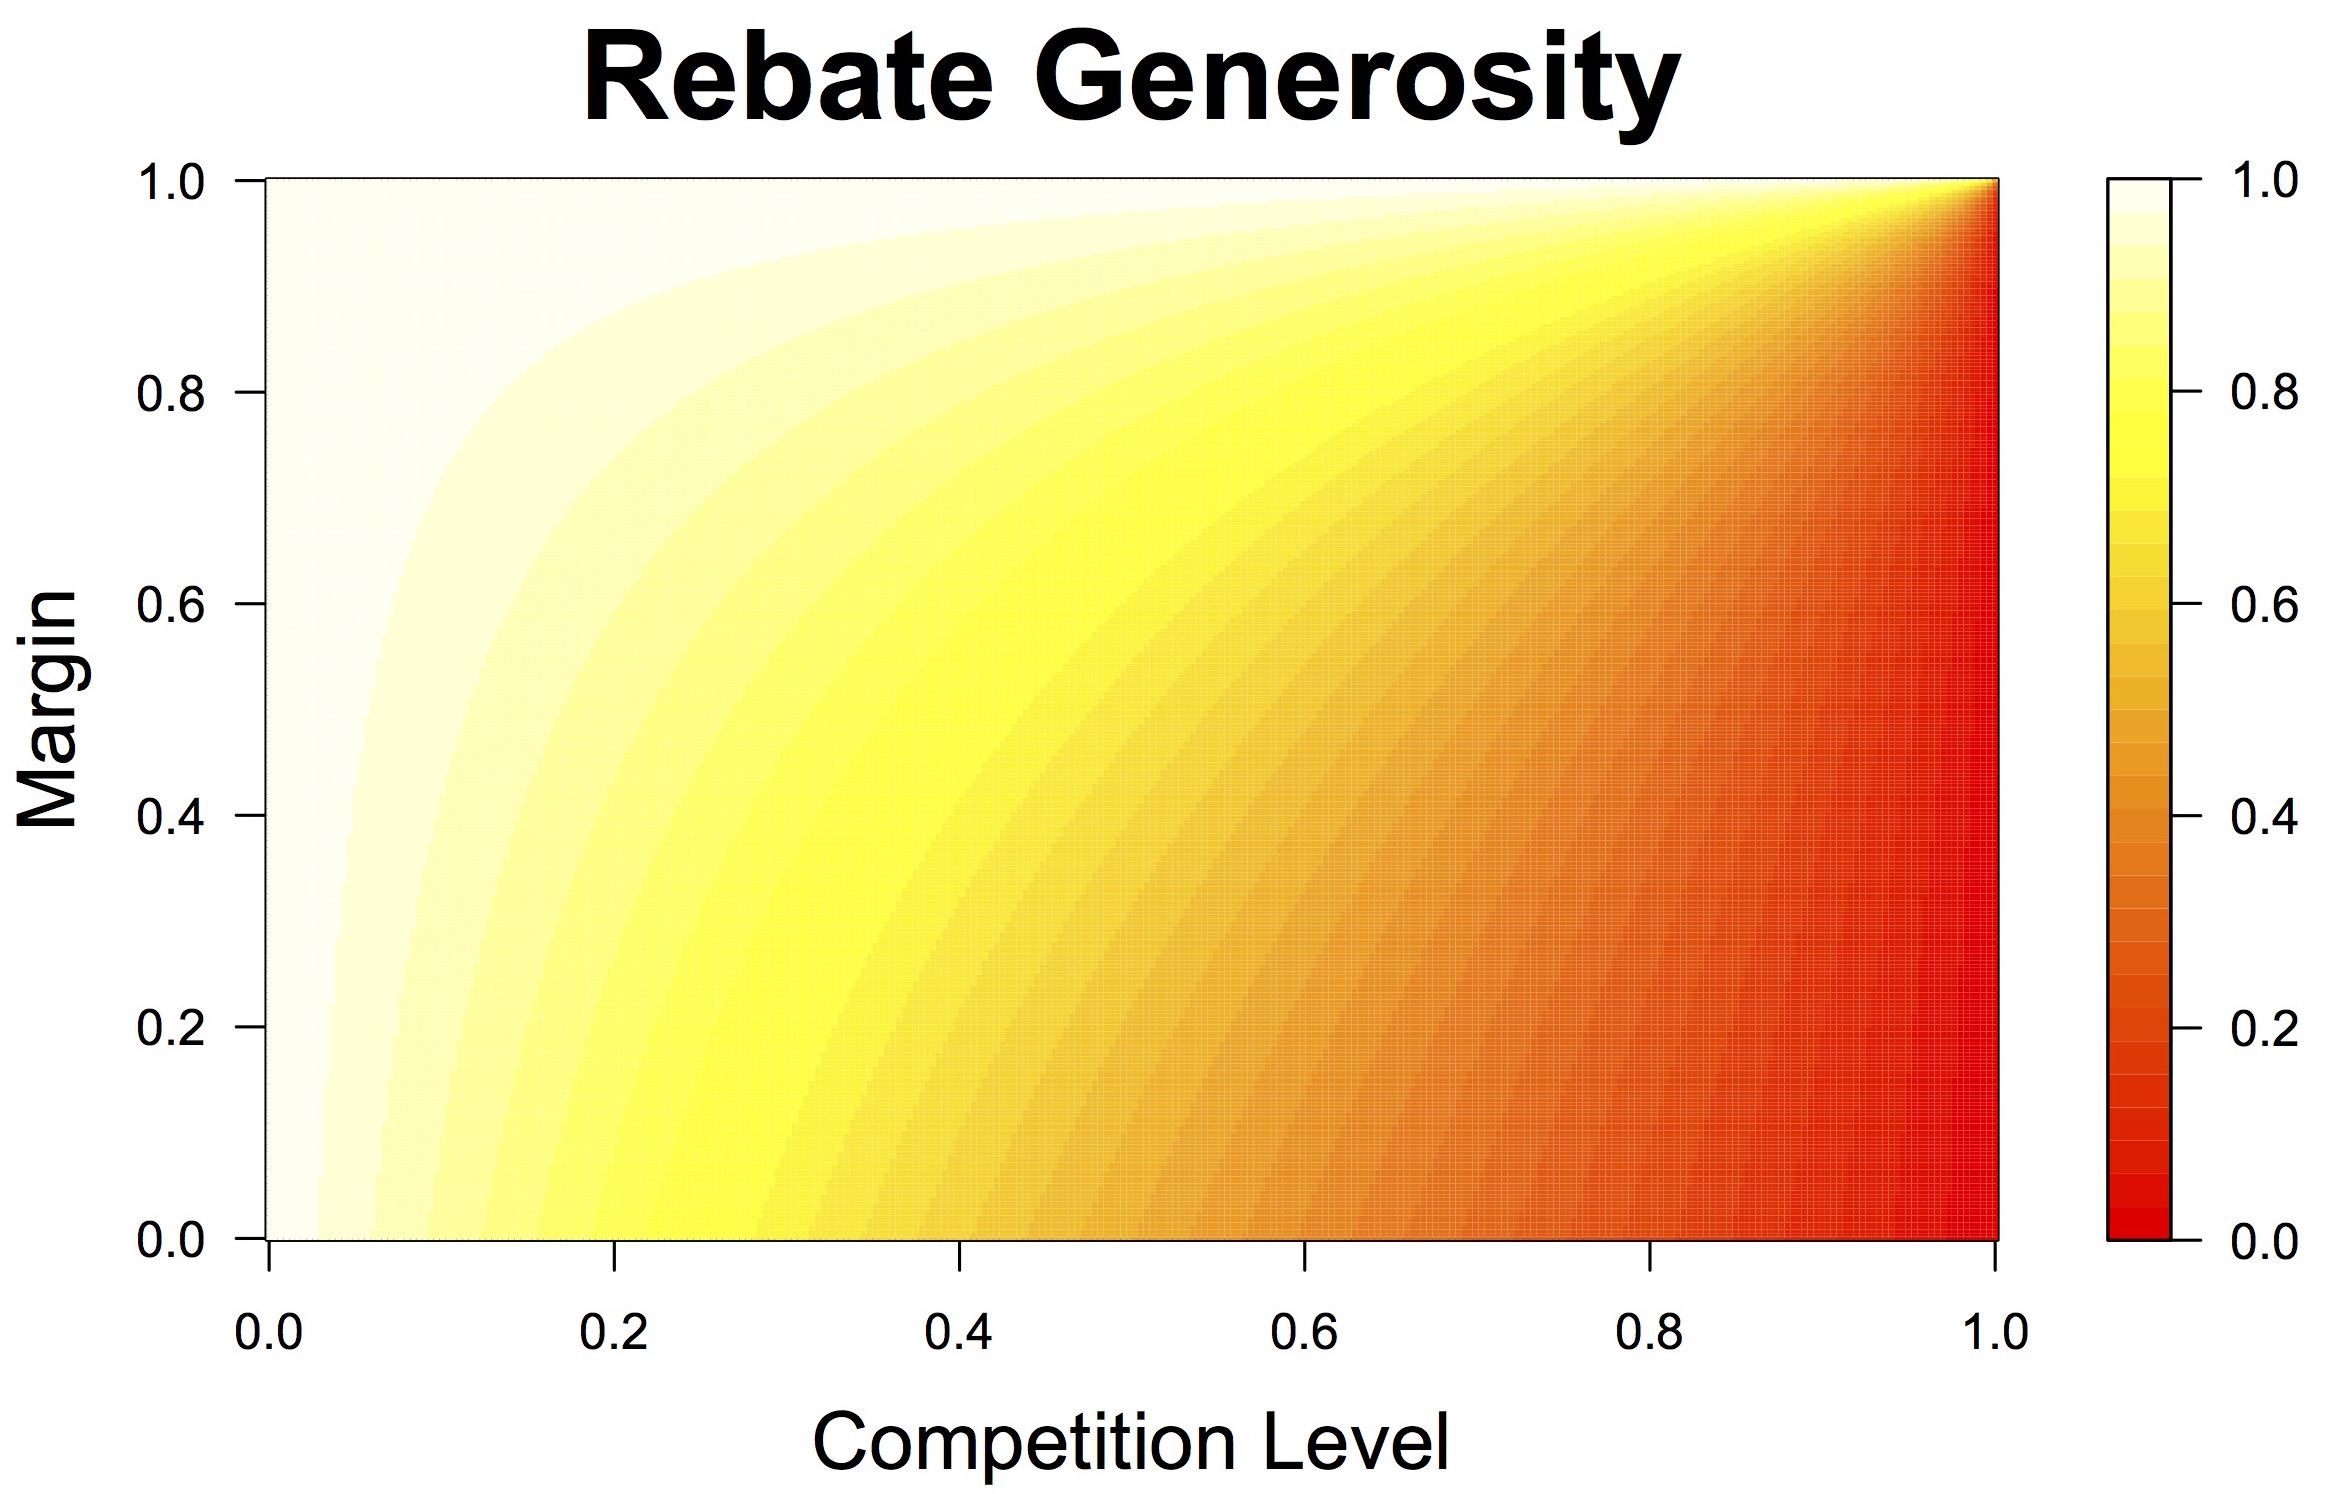
\includegraphics[width = .8\textwidth]{RebateGenerosity_Stretched.jpg}}
\caption{The generosity of rebates, as a function of the margin of the product and the level of competition in the marketplace. The supplier offers a near-complete rebate whenever the market is not competitive or the margin is high. In very competitive markets, rebates are small to non-existent.} \label{fig:rebategenerosity}
\end{figure}



\begin{remark}
There are several interesting observations. First, the optimal order quantity is independent of the level of competition $C$, and the optimal rebate level is independent of the margin $M$.  Second, the ``rebate generosity"  $r/(w+c_h)$ (that is, the fraction of the supplier's costs that can be recovered when inventory goes unsold) is decreasing in $C$ and increasing in $M$. In particular, if the margin is high or the level of competition is low, then the supplier offers a near-complete rebate. As the level of competition rises, both wholesale prices and rebate generosity fall, reaching $w = c_m$ and $r = 0$ in competitive markets. These trends are depicted in Figure \ref{fig:rebategenerosity}.

While it may sound obvious that in a competitive market, wholesale prices fall to the marginal cost $c_m$, this is not immediate, as it is plausible that another supplier could ``undercut" by offering a slightly higher price with a more generous rebate.
\end{remark}


\section{References}

\begin{enumerate}
\item \url{https://www.npr.org/templates/story/story.php?storyId=91461568}
\item \url{https://www.macmillanlearning.com/catalog/page/bookstore-programs}
\end{enumerate}
%\section{Exogenous Overage/Underage Costs}
%
%A retailer faces a classical Newsvendor model, with given overage and underage costs $c_o$ and $c_u$ (presumably determined in part by exogenous prices), and a known demand distribution $D$. A supplier makes profit $\Pi$ on each sale to the retailer, and has the option of offering a rebate $r = \alpha c_o$ for each unsold piece of inventory.
%
%Given $R$ (alternatively, $\alpha$), the retailer will choose order quantity $q(\alpha) = F^{-1}\left( \frac{c_u}{c_u + (1 - \alpha) c_o} \right)$, and the supplier makes profit 
%\[\Pi q(\alpha) - \alpha c_o E_{d \sim F}[(q(\alpha)-d)_+] = \Pi q(\alpha) - \alpha c_o \int_0^{q(\alpha)} F(x)dx.\] If $\alpha = 0$, the retailer chooses $q = q_0$ such that $F(q_0) = \frac{c_u}{c_u+c_o}$. We can change variables so that the supplier optimizes over the order quantity $q(\alpha)$ and is solving the following problem:
%\[ \max_{q \geq q_0} \Pi q - \left(c_o - c_u \frac{1 - F(q)}{F(q)} \right) \int_0^q F(x) dx.\]
%
%\section{Endogenizing Wholesale Prices}
%
%
%\begin{remark}
%The model above is inelegant, because the supplier can offer to compensate for extra inventory, but not to mitigate cost of lost sales. As a result, order quantity is always weakly higher than ``default" quantity $q_0$. This seems somewhat realistic: lost sales are hard to verify (hard to write a contract on), and besides, the supplier presumably has an incentive to sell more. However, we get a more elegant model if we endogenize the wholesale price (and hence overage and underage costs). In this section, we continue to assume that the retail price (MSRP) is fixed.
%\end{remark}
%
%The model is as above, except that $\Pi, c_o, c_u$ are jointly determined by the wholesale price $w$. We assume a fixed retail price $p$ and a constant marginal cost of production and shipping $c_m$ and a constant holding cost $c_h$. %It should be without loss of generality to assume $p = 1$ and $c = 0$.




%\begin{remark}
%This is the familiar monopoly problem. It may seem a bit unexpected, as $D$ is a distribution of number of customers, not their willingness to pay. But the retailer's willingness to pay for the $q^{th}$ item is exactly $p$ times the probability that it sells, minus holding costs.
%\end{remark}



%\begin{remark}
%What happens if we add competition among suppliers offering a homogeneous product? Intuitively, with many suppliers, the lowest-cost supplier should win the contract, but should have to provide enough utility to the retailer that it is not profitable for the retailer to deviate to another supplier. Thus, a reduced form way to capture the competition is to assume that the retailer has an outside option $\Pi$.
%\end{remark}






\begin{comment}

\subsection{ Extensions}

Sanity Checks:
\begin{itemize}
\item Lower margin (higher manufacturing/shipping costs) implies higher $w$, but lower rebate.
\item In a competitive market, $w = c_m$ (the product is offered at marginal cost), with no rebate. (Latter part not so obvious -- maybe I could attract customers by offering higher prices, but higher rebate)
\item More competition implies lower prices.
\end{itemize}


\begin{remark}
Could consider a model with separate manufacture and shipping costs, and some salvage value (to the publisher) for unsold books. Not clear whether this will offer any new insights. Perhaps if some suppliers are close but with high manufacturing costs, some are far (large shipping costs) but low manufacturing costs, and the retailer can purchase from multiple suppliers.
\end{remark}

We could assume that the supplier can impose minimum order quantities, but given that the retailer has no private information, they will always get zero surplus in this case.

\end{comment}

\end{document}  